\section{Results}
\subsection{2D Tetris}
\subsection{3D Tetris}
We trained a DQN agent to play a 3D Tetris Battle environment through a step-by-step complexity escalation. Initially, training began with a simplified setup where the agent controlled only the placement position of the basic square-shaped tetromino. Subsequently, we introduced rotational movements while maintaining the single square-shaped piece. Finally, the complexity was increased by incorporating multiple tetromino shapes with both positional and rotational actions.

The following detailed results pertain specifically to the final training scenario involving multiple shapes with both placement and rotation capabilities. The DQN utilized an epsilon-greedy strategy for exploration, with the training curve illustrated in Figure~\ref{fig:training_curve}. After approximately 4000 episodes, epsilon reached its minimal exploration rate of 0.001, and the overall game scores began to rise steadily. Due to inherent randomness in the Tetris environment, the scores exhibited considerable variability throughout training. Nevertheless, the agent achieved its peak performance at episode 6689, attaining a maximum score of 20,369 and clearing 731 planes.

We then evaluated this best-performing model through 10 inference runs. The average score during these evaluations was 3945.2 points, with an average of 128.2 planes cleared per game. In stark contrast, a random agent averaged only 21.9 points, demonstrating significant improvement and the efficacy of our trained DQN model. Observations from the inference process revealed strategic gameplay, with the agent effectively planning plane clearances, utilizing rotations to fill gaps optimally, and positioning elongated tetrominoes strategically at the edges to minimize height variations.

An example inference video demonstrating the agent’s performance is available at the following URL: \url{[https://drive.google.com/file/d/1d25D7g1W9oFewgXVb2cX2vHWCRS6xZln/view?usp=sharing]}.

\begin{figure}[htbp]
    \centering
    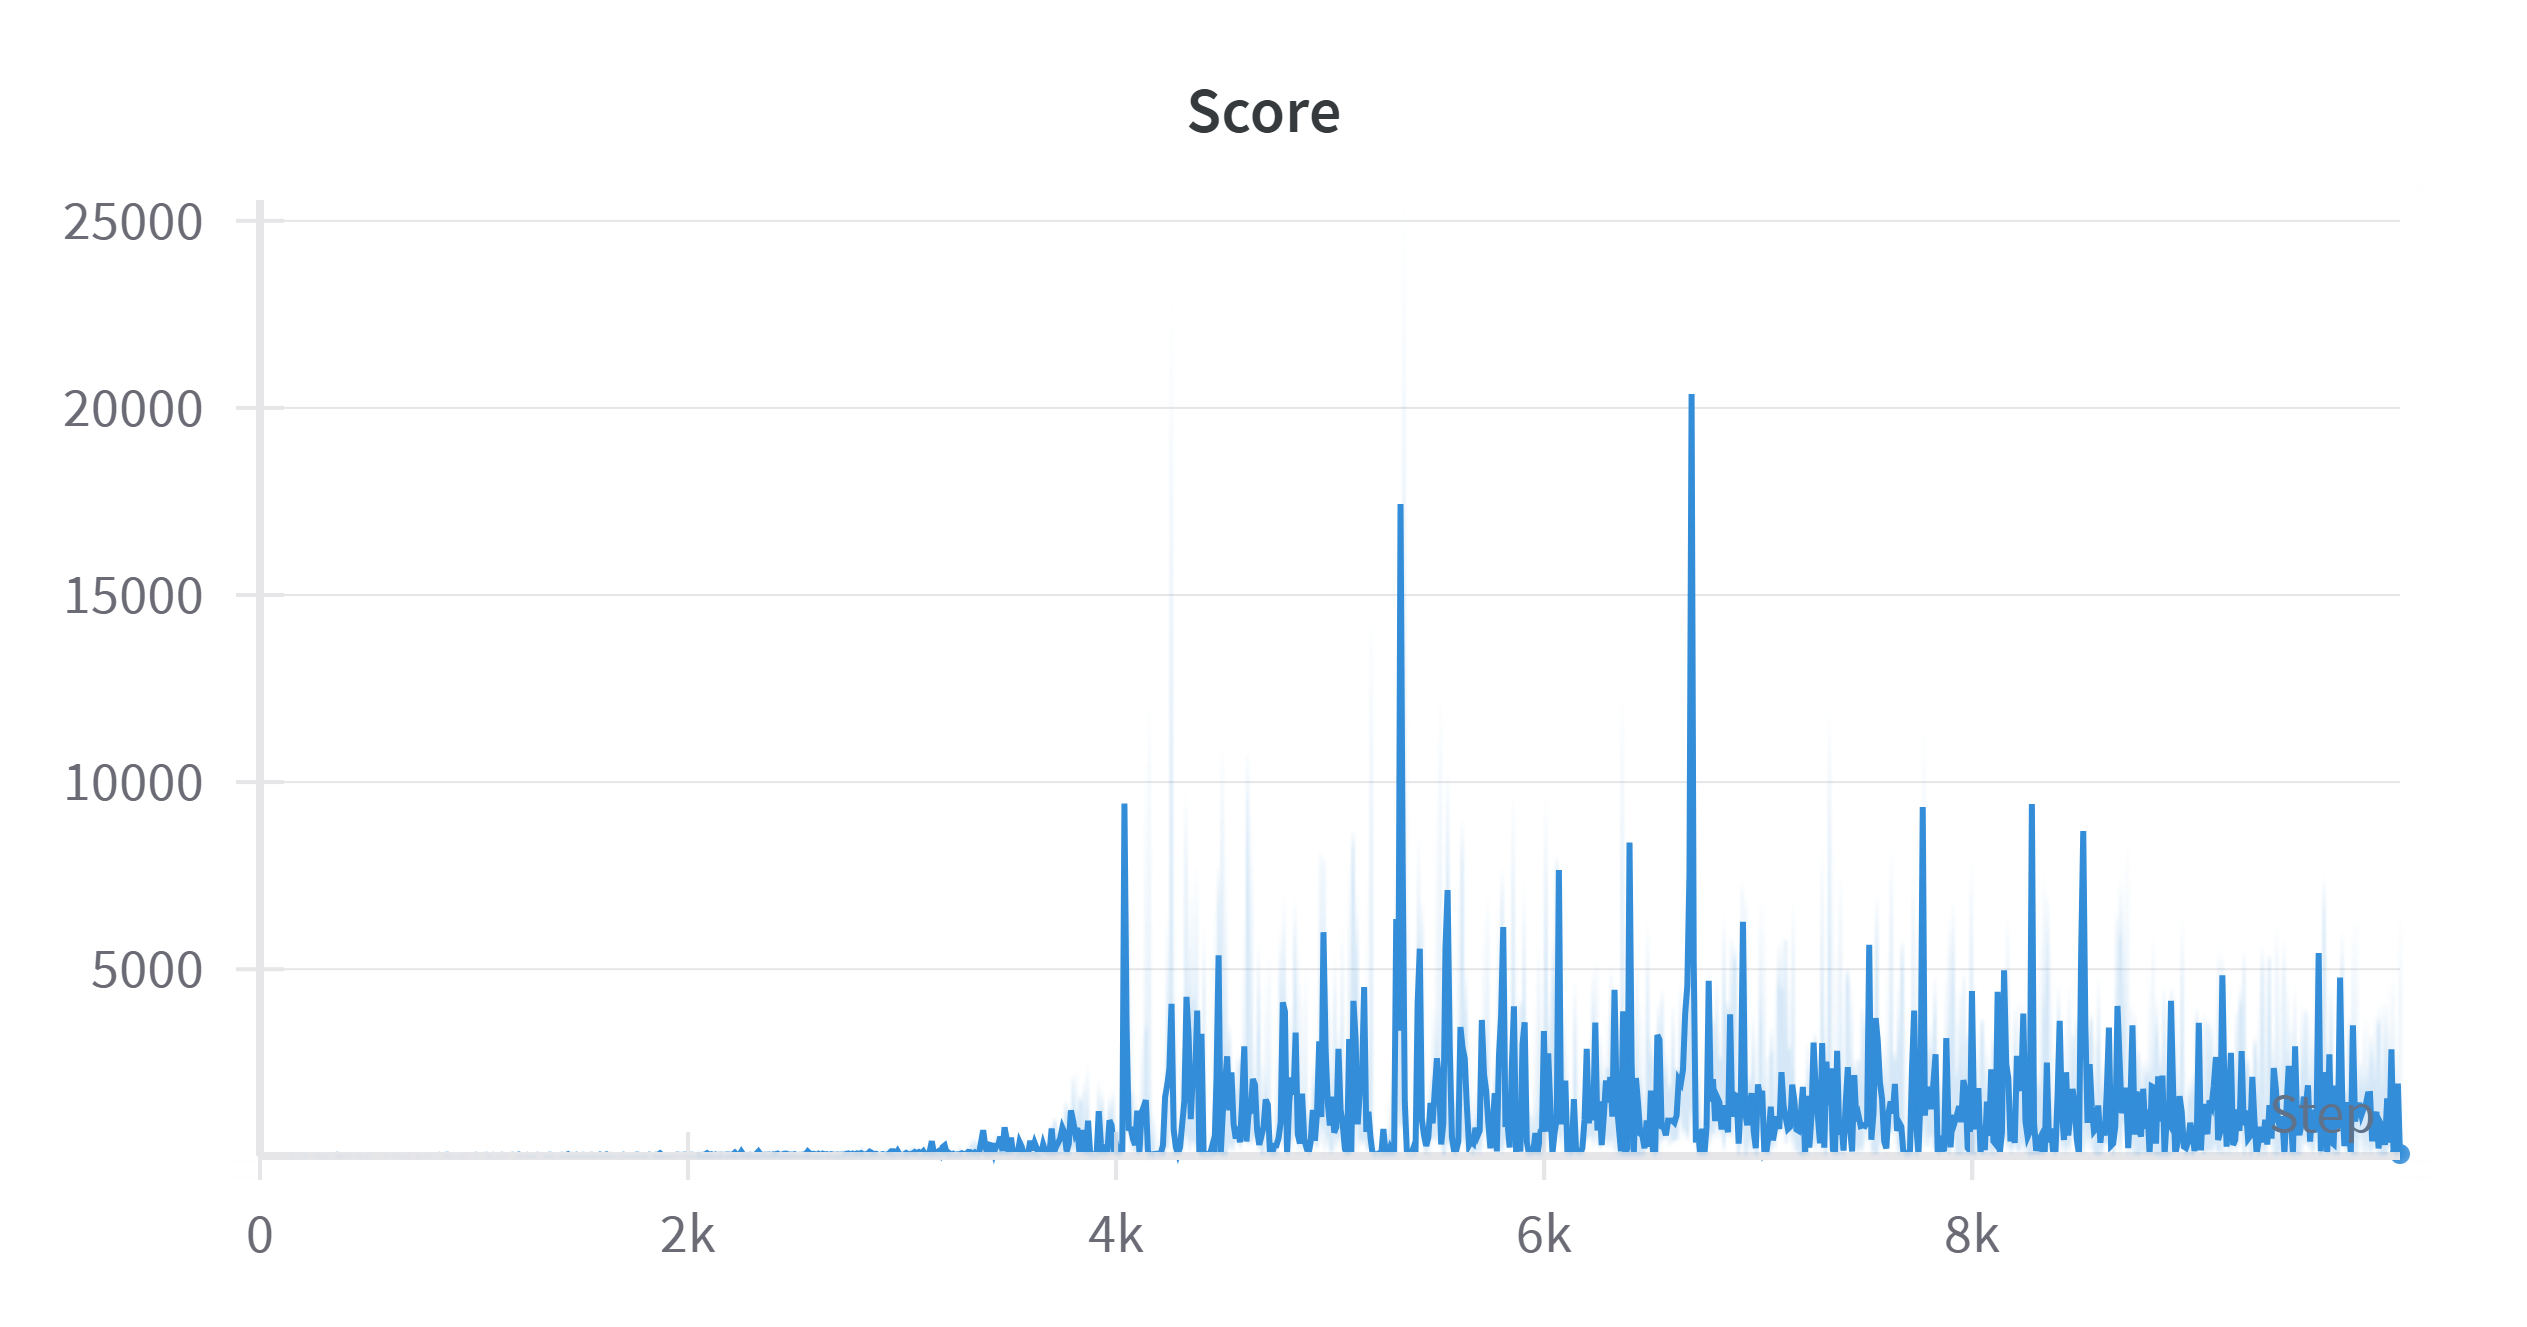
\includegraphics[width=0.8\textwidth]{./images/score_history.png}\\[0.5cm]
    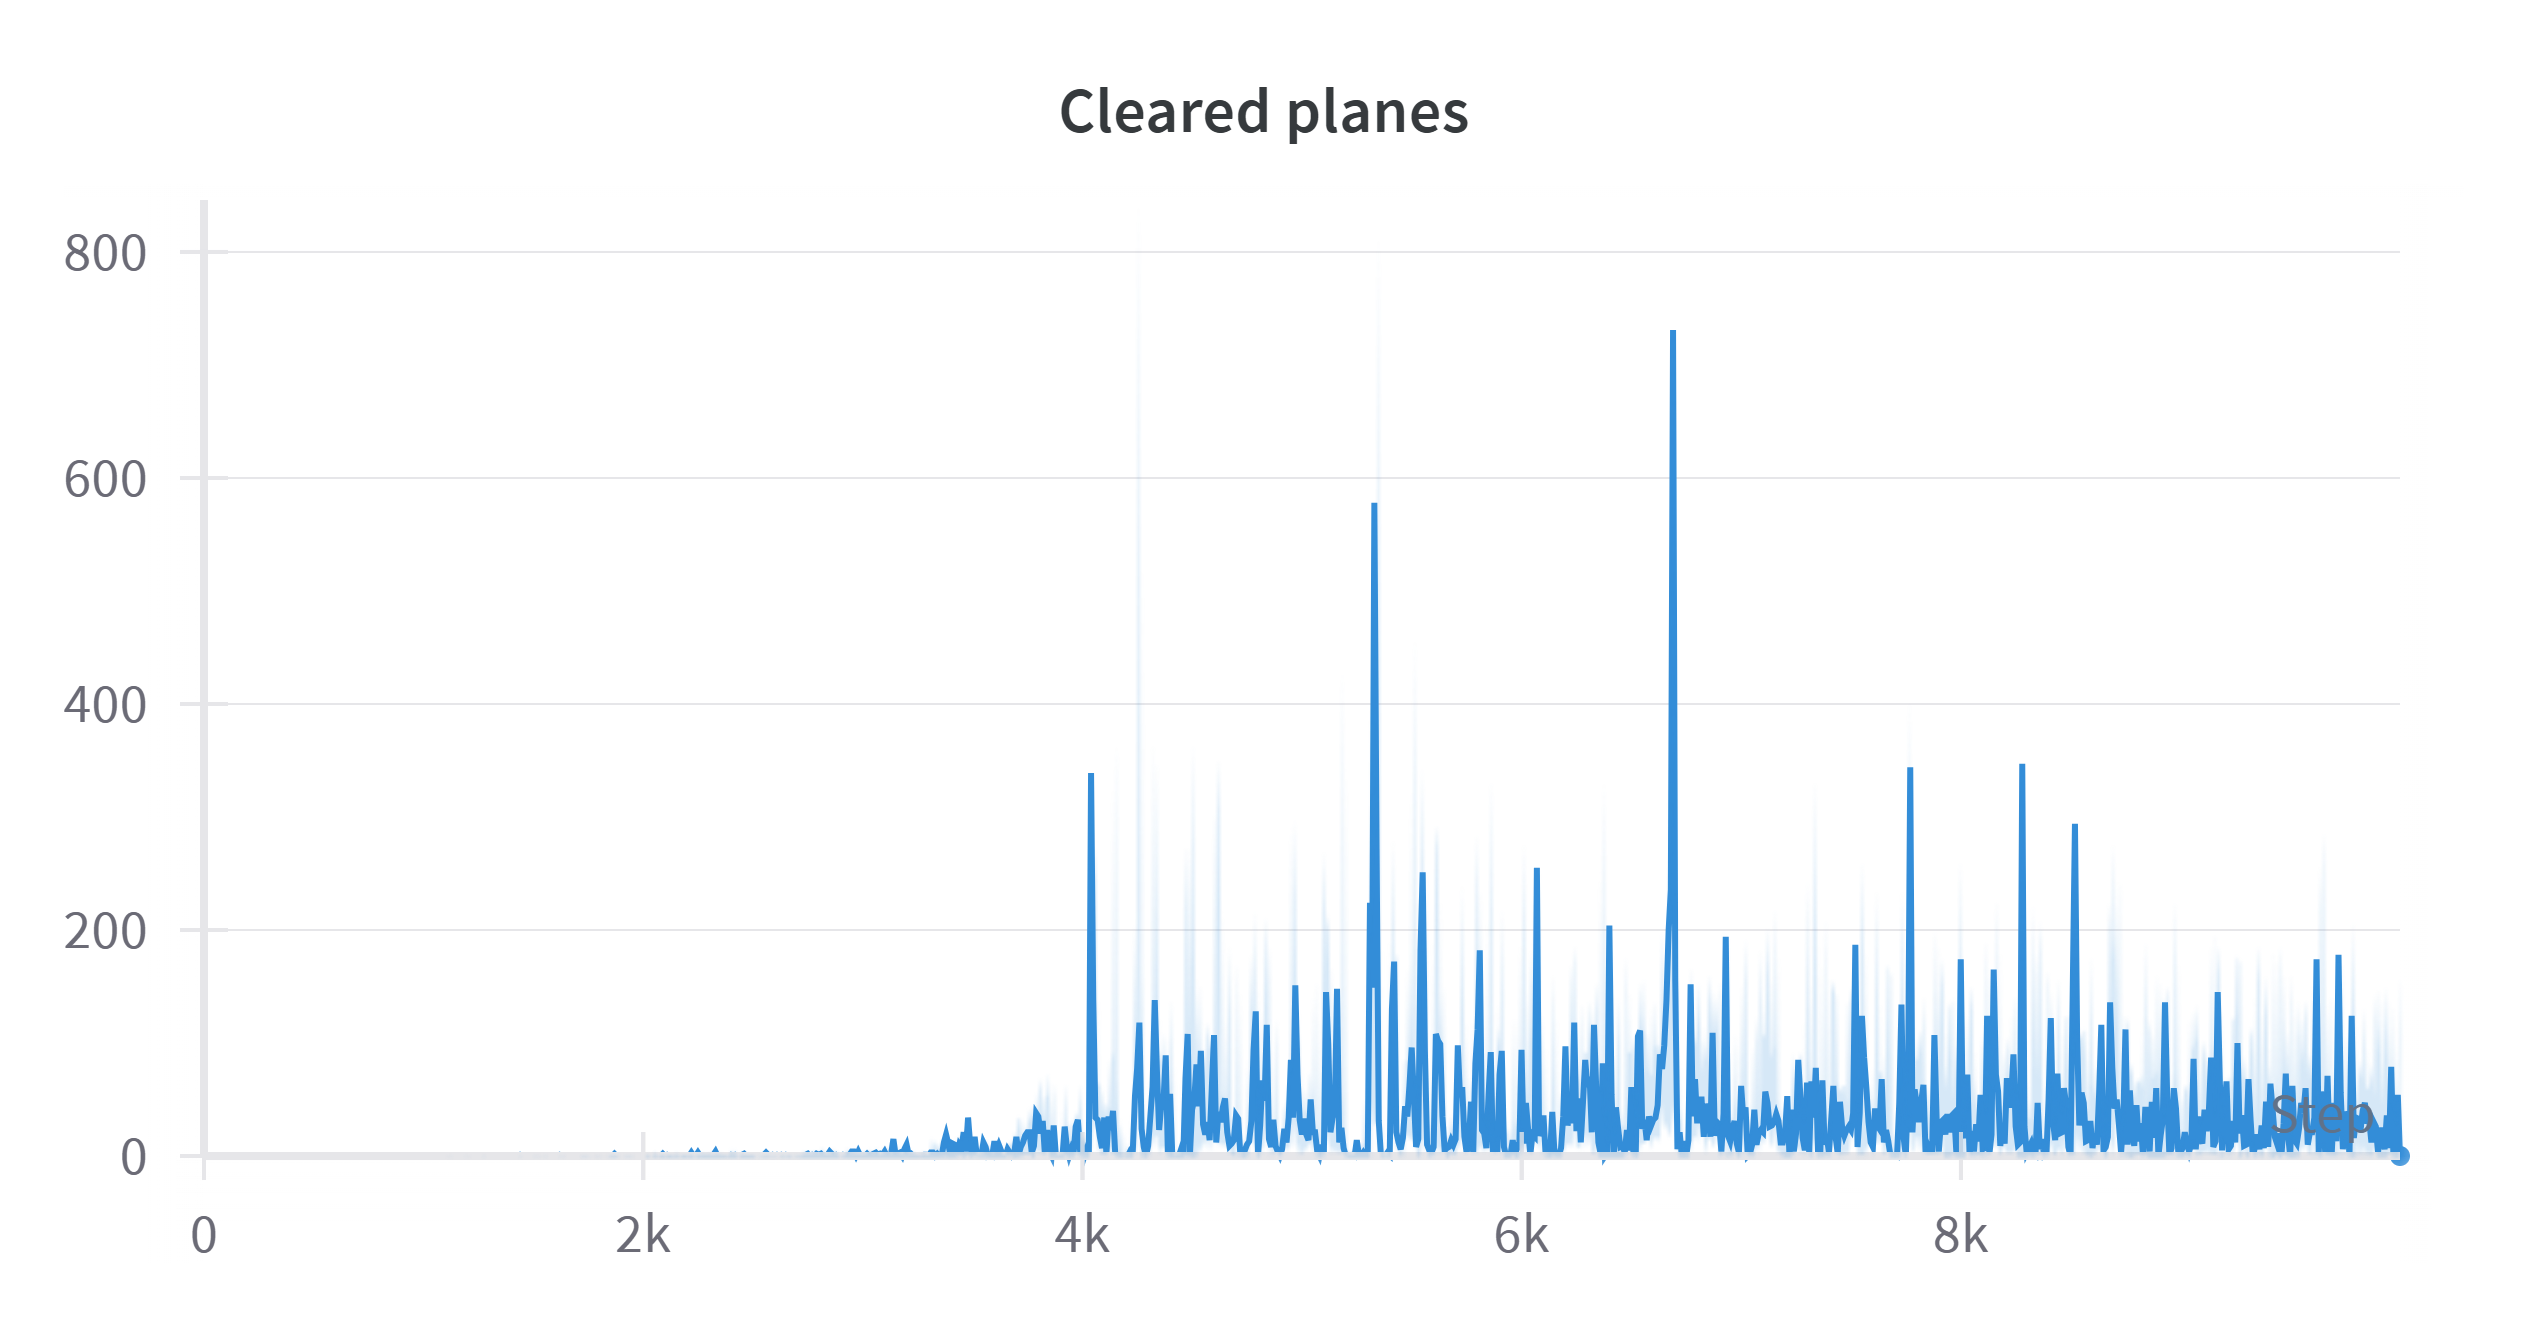
\includegraphics[width=0.8\textwidth]{./images/cleared_planes.png}
    \caption{Training curves of the DQN agent in the 3D Tetris Battle environment. The upper plot shows the game scores over training episodes. The lower plot illustrates the number of planes cleared per episode, indicating an overall improvement in the agent's strategic gameplay.}
    \label{fig:training_curve}
\end{figure}